% Reporte de la actividad 3A — Implementación y comparación de índices de vecinos más cercanos
% Compilación: latexmk -pdf -jobname=Reporte_Actividad3A reporte.tex
% Las cifras provienen de results/*.csv y las figuras de figures/ (generadas por el notebook).
% Límite de la actividad: máximo tres páginas.
\documentclass[10pt,a4paper]{article}

\usepackage[T1]{fontenc}
\usepackage[utf8]{inputenc}
\usepackage[spanish,es-nodecimaldot]{babel}
\usepackage[margin=1.7cm,top=1.5cm,bottom=1.6cm]{geometry}
\usepackage{amsmath}
\usepackage{booktabs}
\usepackage{array}
\usepackage{xcolor}
\usepackage{microtype}
\usepackage{enumitem}
\usepackage{graphicx}
\usepackage{float}
\usepackage[font=small,labelfont=bf,skip=2pt]{caption}
\usepackage[hidelinks]{hyperref}

\graphicspath{{figures/}}

\definecolor{acento}{HTML}{1F6FEB}
\definecolor{cLSH}{HTML}{2A78D6}
\definecolor{cPQ}{HTML}{EB6834}
\definecolor{cHNSW}{HTML}{1BAF7A}
\definecolor{cEx}{HTML}{555555}
\newcommand{\term}[1]{\textcolor{acento}{\texttt{#1}}}
\newcommand{\famsq}[1]{\textcolor{c#1}{\rule{0.6em}{0.6em}}}

\setlist[itemize]{topsep=1pt,itemsep=0pt,parsep=0pt,leftmargin=1.2em}
\setlist[enumerate]{topsep=1pt,itemsep=0pt,parsep=0pt,leftmargin=1.5em}
\setlength{\parskip}{2pt}
\setlength{\textfloatsep}{6pt}
\setlength{\floatsep}{6pt}
\setlength{\intextsep}{5pt}
\renewcommand{\arraystretch}{1.02}
\usepackage{titlesec}
\titlespacing*{\section}{0pt}{5pt}{2pt}
\titlespacing*{\paragraph}{0pt}{3pt}{0.6em}

\title{\vspace{-1.5cm}\textbf{Índices de vecinos más cercanos aproximados}\\[2pt]
\large Compromiso exactitud--tiempo--memoria de LSH, IVF-PQ y HNSW}
\author{David Segundo García}
\date{\vspace{-0.3cm}Actividad 3A \textperiodcentered\ 28 de septiembre de 2026
\textperiodcentered\ acompaña al notebook \texttt{Actividad3A\_Indices\_ANN.ipynb}}

\begin{document}
\maketitle
\vspace{-0.9cm}

\section{Montaje experimental}

\paragraph{Colecciones.} \emph{Embeddings} de palabras \textbf{GloVe 6B} de 100 dimensiones
(Stanford NLP; Wikipedia 2014 + Gigaword 5). De las 101\,000 palabras más frecuentes se apartaron
1\,000 al azar como consultas no indexadas. Las 100\,000 restantes forman la colección
\textbf{100k} (38.15~MB) y una muestra aleatoria de ellas la colección \textbf{10k} (3.81~MB), con
10k $\subset$ 100k y la misma distribución. Los vectores son \texttt{float32} con norma $L_2=1$.

\paragraph{Métrica y línea base.} Se usa la \textbf{distancia coseno}, porque en los
\emph{embeddings} de palabras el significado está en la dirección y la norma refleja la frecuencia.
Con vectores unitarios, $\lVert x-y\rVert^2 = 2\,d_{\cos}(x,y)$, así que $L_2$, producto interno y
coseno dan el mismo orden de vecinos. Eso permite usar índices $L_2$ (IVF-PQ) y es la hipótesis del
LSH de hiperplanos (SimHash). La referencia exacta es una fuerza bruta con NumPy, verificada contra
\texttt{faiss.IndexFlatIP} con concordancia de 1.000, y de ella sale el \emph{ground truth} del
recall@10.

\paragraph{Índices y medición.} Se implementaron las tres familias y se barrieron dos
hiperparámetros por índice (72 configuraciones por colección):

\begin{table}[H]
\centering\footnotesize
\begin{tabular}{@{}lll@{}}
\toprule
\textbf{Familia} & \textbf{Implementación} & \textbf{Barrido (estructural $\times$ de consulta)} \\
\midrule
\famsq{LSH}~LSH & \texttt{faiss.IndexLSH} + reordenamiento exacto (\texttt{IndexRefineFlat}) &
\texttt{nbits} $\in\{64\ldots512\}$ $\times$ \texttt{k\_factor} $\in\{1\ldots100\}$ \\
\famsq{PQ}~IVF-PQ & \texttt{faiss.IndexIVFPQ}, $\texttt{nlist}=2\sqrt{N}$, 8 bits por subvector &
\texttt{M} $\in\{10,20,50\}$ B/vector $\times$ \texttt{nprobe} $\in\{1\ldots128\}$ \\
\famsq{HNSW}~HNSW & \texttt{hnswlib}, \texttt{ef\_construction}~=~200, \texttt{space='ip'} &
\texttt{M} $\in\{8\ldots48\}$ $\times$ \texttt{ef\_search} $\in\{10\ldots640\}$ \\
\bottomrule
\end{tabular}
\end{table}

Las 1\,000 consultas se ejecutan una a una en \textbf{un solo hilo} (Apple M5). Se reportan la
latencia media y el p95, y la memoria como el tamaño del índice serializado, que incluye los
vectores originales cuando el índice los guarda.

\section{Compromiso exactitud--tiempo--memoria}

\begin{figure}[H]
\centering
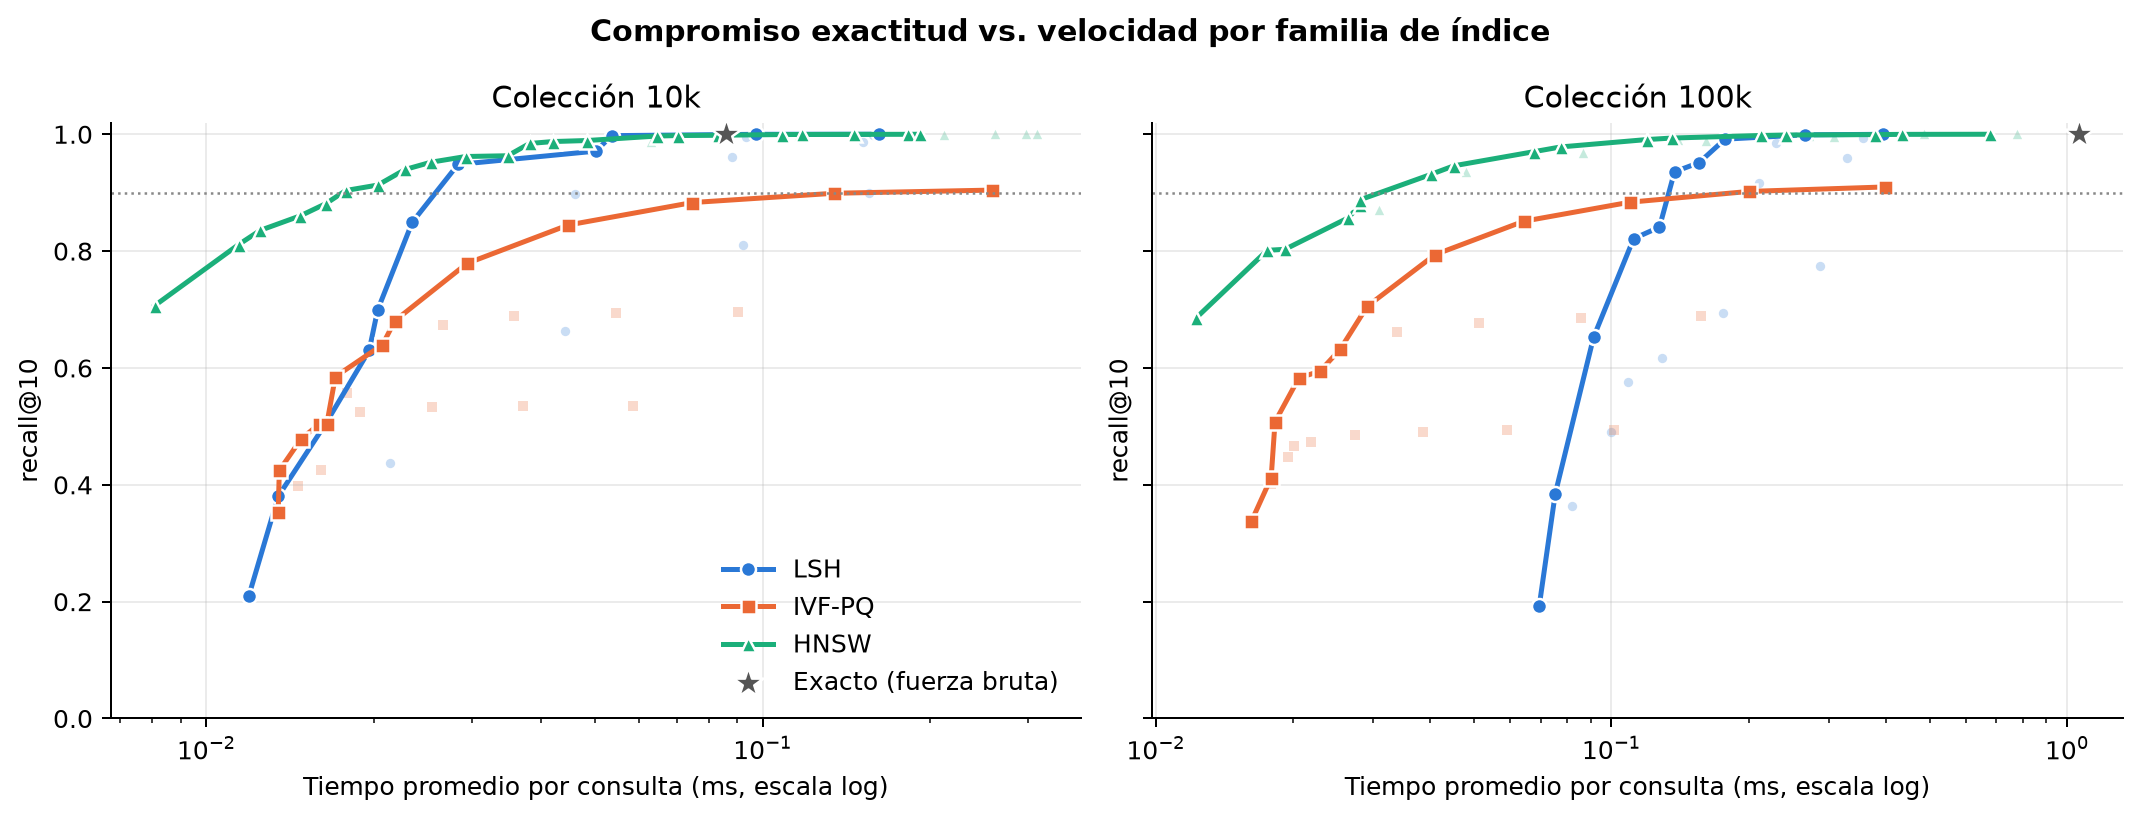
\includegraphics[width=0.94\linewidth]{tradeoff_recall_time.png}
\caption{Frontera de Pareto recall@10 vs.\ latencia por familia. Los puntos tenues son
configuraciones dominadas, la estrella es la búsqueda exacta y la línea punteada el requisito 0.90.}
\end{figure}

\paragraph{HNSW domina la frontera} en ambas colecciones. En 100k alcanza recall 0.970 en
0.068~ms y 0.999 en 0.38~ms, frente a 1.06~ms de la fuerza bruta. A cambio, es el que más memoria
usa: con $M=32$ el grafo añade $\approx$276~B por vector (64.5~MB contra 38.1~MB de los datos
crudos) y el que más tarda en construirse (4.3~s).
\textbf{IVF-PQ es el más compacto.} Con $M=50$ ocupa 5.9~MB, 6.5$\times$ menos que los datos y
11$\times$ menos que HNSW. Pero la cuantización impone un \textbf{techo de recall que no depende de
\texttt{nprobe}}: $\approx$0.49 con $M=10$, $\approx$0.69 con $M=20$ y $\approx$0.91 con $M=50$.
Las distancias ADC no alcanzan a separar vecinos tan cercanos como los de GloVe.
\textbf{LSH necesita los vectores originales.} Con solo el código binario
(\texttt{k\_factor}~=~1) llega a 0.62 con 512 bits. Para superar 0.90 debe reordenar candidatos con
los vectores \texttt{float32}, y entonces su memoria (44.4~MB) supera a la de los datos. Además,
\texttt{IndexLSH} recorre todos los códigos, así que su costo sigue siendo $O(N)$.

\begin{figure}[H]
\centering
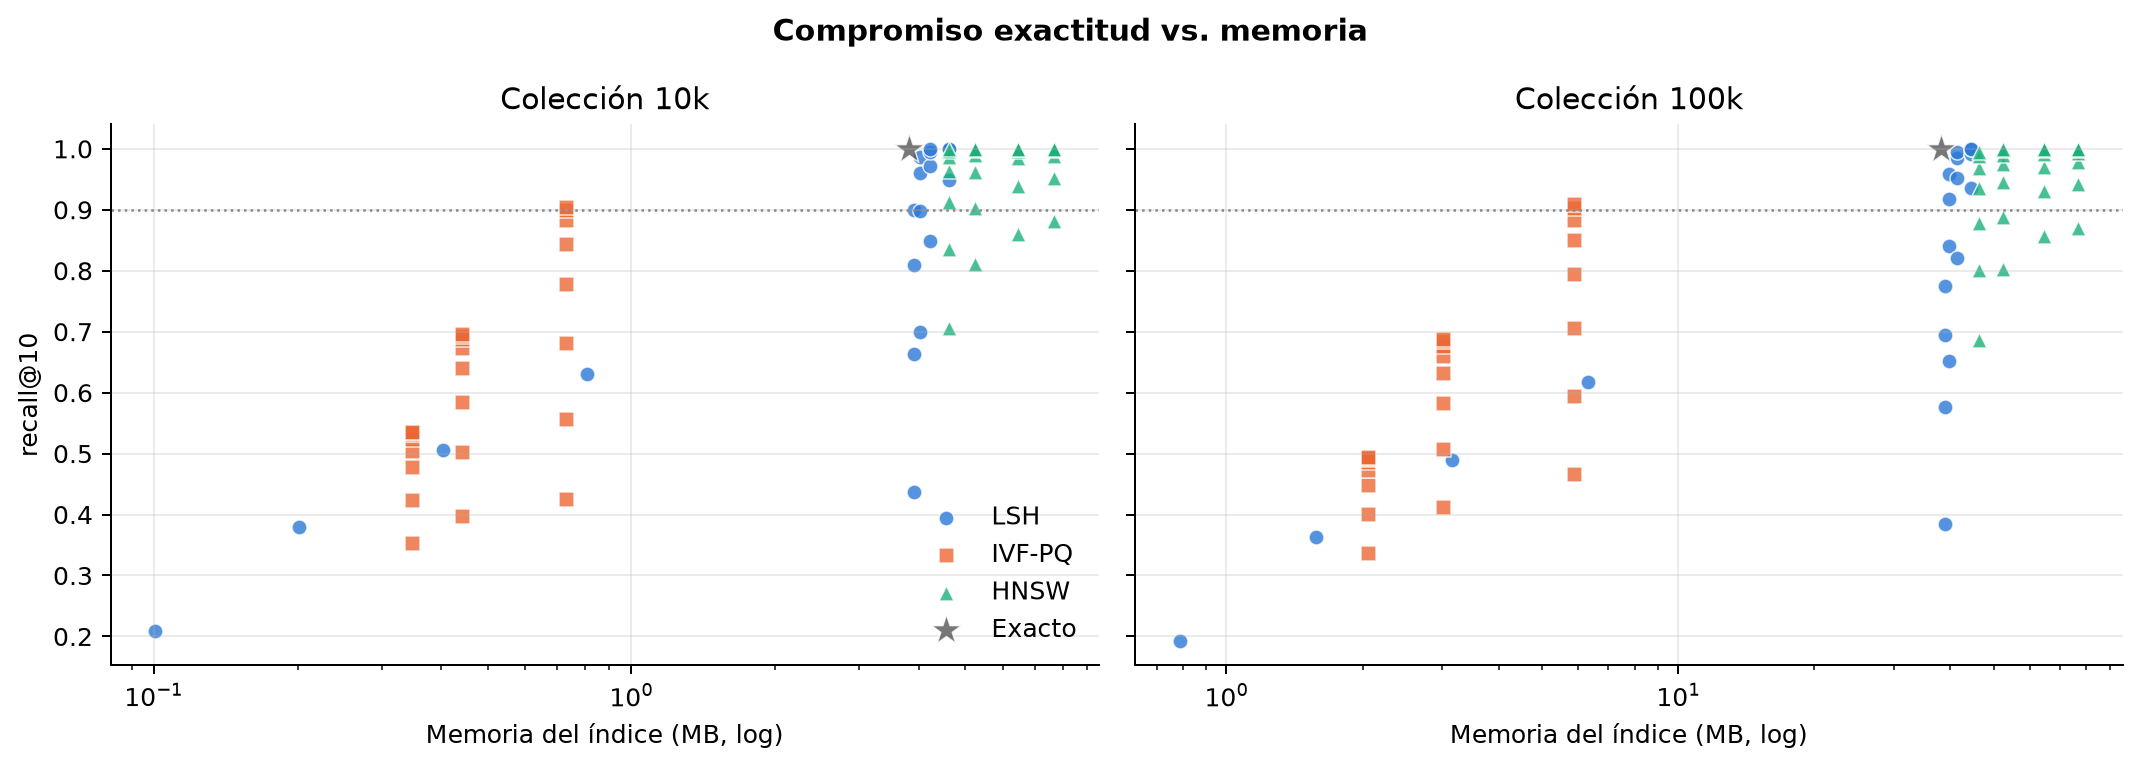
\includegraphics[width=0.86\linewidth]{tradeoff_recall_memory.png}
\caption{Recall@10 vs.\ memoria del índice (escala log). IVF-PQ es la única familia que cumple
0.90 por debajo del tamaño de los datos crudos (estrella).}
\end{figure}

\section{Punto de operación: recall@10 $\geq$ 0.90 al menor costo}

\textbf{Escenario:} buscador semántico en línea (sugerencia y expansión de términos) con una
consulta por petición. \textbf{Requisito:} recall@10 $\geq 0.90$. \textbf{Criterio:} entre las
configuraciones que cumplen, la de menor latencia media; si hay empate de $\pm$5\,\%, la de menor
memoria.

\begin{table}[H]
\centering\small
\begin{tabular}{@{}llcccccr@{}}
\toprule
\textbf{Col.} & \textbf{Índice} & \textbf{Configuración} & \textbf{recall} & \textbf{ms (p95)} &
\textbf{MB} & \textbf{Constr. (s)} & \textbf{Acel.} \\
\midrule
10k  & \famsq{Ex}~Exacto   & fuerza bruta             & 1.000 & 0.086 (0.114) & 3.81  & ---  & 1.0$\times$ \\
10k  & \famsq{HNSW}~HNSW   & \texttt{M=16, ef=20}      & 0.904 & 0.018 (0.023) & 5.24  & 0.21 & \textbf{4.8$\times$} \\
10k  & \famsq{LSH}~LSH     & \texttt{nbits=512, kf=5}  & 0.948 & 0.028 (0.030) & 4.62  & 0.01 & 3.0$\times$ \\
10k  & \famsq{PQ}~IVF-PQ   & \texttt{M=50, nprobe=128} & 0.904 & 0.258 (0.298) & \textbf{0.73} & 0.81 & 0.3$\times$ \\
\midrule
100k & \famsq{Ex}~Exacto   & fuerza bruta             & 1.000 & 1.063 (1.325) & 38.15 & ---  & 1.0$\times$ \\
100k & \famsq{HNSW}~HNSW   & \texttt{M=32, ef=20}      & 0.931 & 0.040 (0.055) & 64.50 & 4.29 & \textbf{26.5$\times$} \\
100k & \famsq{LSH}~LSH     & \texttt{nbits=512, kf=5}  & 0.936 & 0.138 (0.145) & 44.45 & 0.06 & 7.7$\times$ \\
100k & \famsq{PQ}~IVF-PQ   & \texttt{M=50, nprobe=64}  & 0.902 & 0.200 (0.211) & \textbf{5.88} & 1.82 & 5.3$\times$ \\
\bottomrule
\end{tabular}
\caption{Puntos de operación por menor latencia (\texttt{results/operating\_points.csv}).}
\end{table}

\paragraph{Justificación con los datos.}
\begin{itemize}
  \item \textbf{HNSW (100k).} \texttt{M=32, ef=20} es la configuración más rápida que cumple (0.931
        en 0.040~ms). Con menos aristas, \texttt{M=16, ef=20} se queda en 0.888. La opción que cumple
        con menos memoria (\texttt{M=8, ef=80}, 46.3~MB) es un 20\,\% más lenta.
  \item \textbf{LSH.} Con 512 bits basta reordenar $5\times10$ candidatos (0.936). Con 256 o 128 bits
        hacen falta \texttt{k\_factor} de 20 o 50 y la latencia sube a 0.156 y 0.211~ms.
  \item \textbf{IVF-PQ.} Solo $M=50$ cumple, y por poco: con \texttt{nprobe=32} se queda en 0.884.
        En 10k necesita \texttt{nprobe=128} de 200 celdas, es decir, recorrer el 64\,\% de la base;
        por eso resulta 3$\times$ \emph{más lento} que la fuerza bruta. Con pocos datos, el costo fijo
        de las tablas ADC y del cuantizador grueso no se amortiza.
\end{itemize}

\section{Escalabilidad: de 10k a 100k vectores (datos $\times$10)}

\begin{figure}[H]
\centering
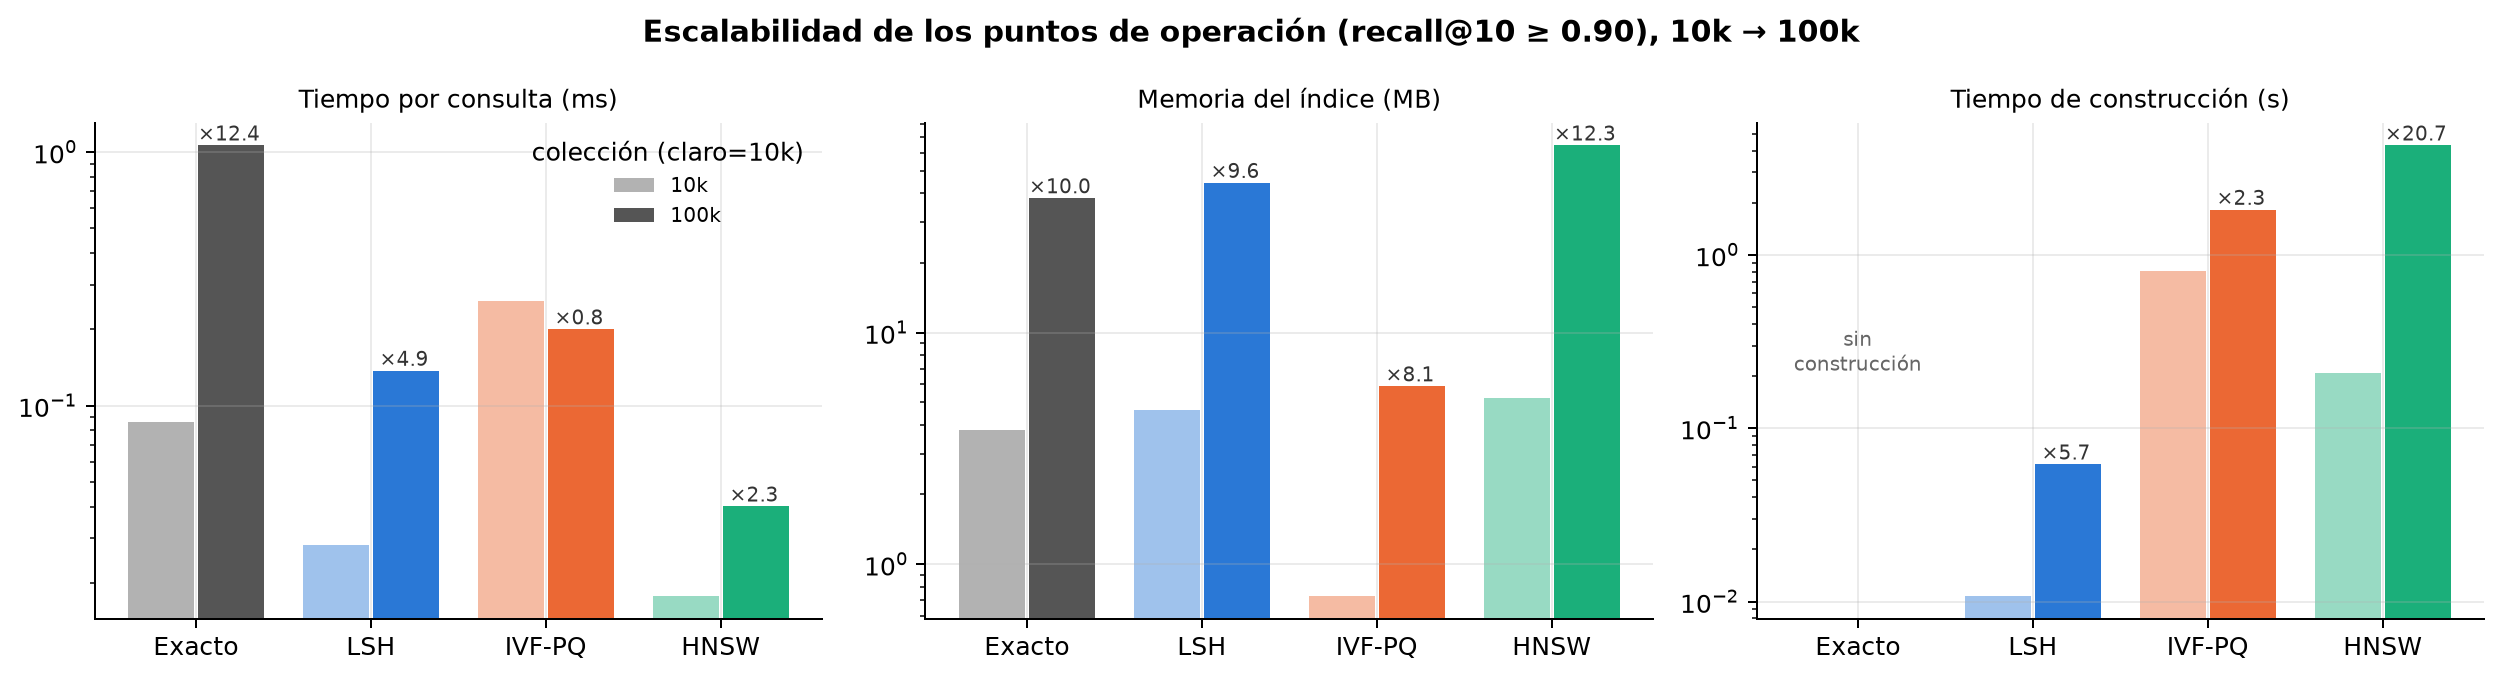
\includegraphics[width=0.94\linewidth]{scalability.png}
\caption{Latencia, memoria y construcción de cada punto de operación en 10k (tono claro) y 100k.}
\end{figure}

\paragraph{Tiempo.} La fuerza bruta crece $\times$12.4, en línea con su costo $O(N\cdot d)$. HNSW
crece solo $\times$2.3, un comportamiento cercano al logarítmico, y su ventaja sobre el exacto sube
de 4.8$\times$ a 26.5$\times$. LSH crece $\times$4.9, porque el escaneo de códigos es lineal. IVF-PQ
incluso \emph{baja} ($\times$0.78): \texttt{nlist} crece con $\sqrt{N}$ y basta explorar una
fracción menor de la base (\texttt{nprobe}/\texttt{nlist} pasa del 64\,\% al 10\,\%).
\textbf{Hiperparámetros.} Para sostener el requisito, HNSW tuvo que pasar de $M=16$ a $M=32$: con la
configuración de 10k, en 100k cae de 0.904 a 0.888. LSH conservó la suya (0.948 $\rightarrow$
0.936). \textbf{Memoria.} Todo crece casi linealmente: el exacto $\times$10, LSH $\times$9.6,
IVF-PQ $\times$8.1 (los centroides son un costo fijo) y HNSW $\times$12.3, en parte por el cambio a
$M=32$. Al escalar, \textbf{el tiempo favorece a HNSW y la memoria a IVF-PQ}.

\section{Recomendación para producción}

\begin{table}[H]
\centering\small
\begin{tabular}{@{}>{\raggedright\arraybackslash}p{3.3cm}>{\raggedright\arraybackslash}p{3.5cm}>{\raggedright\arraybackslash}p{9.9cm}@{}}
\toprule
\textbf{Escenario} & \textbf{Índice recomendado} & \textbf{Por qué (datos medidos en 100k)} \\
\midrule
Baja latencia, RAM suficiente (escenario principal) &
\famsq{HNSW}~HNSW, \texttt{M=32}, \texttt{ef\_search=40} &
\texttt{ef=20} ya cumple (0.931), pero conviene margen frente a la variación entre consultas:
\texttt{ef=40} da 0.970 en 0.068~ms, 15.7$\times$ más rápido que el exacto. \texttt{ef} se ajusta
en caliente sin reconstruir el índice. Costo: 64.5~MB (1.7$\times$ los datos). \\
\addlinespace
Memoria limitada (\emph{edge}, millones de vectores) &
\famsq{PQ}~IVF-PQ, \texttt{M=50}, \texttt{nprobe=64} &
5.9~MB (6.5$\times$ menos que los datos) con recall 0.902 en 0.20~ms. Su techo de $\approx$0.91
puede subir con OPQ o reordenando los candidatos con vectores en disco. \\
\addlinespace
No recomendado como índice principal &
\famsq{LSH}~LSH (\texttt{IndexLSH} + \emph{refine}) &
Es el más barato de construir (0.06~s) y sirve para deduplicación o \emph{streaming}, pero ocupa
más memoria que los datos y su latencia crece linealmente con $N$. \\
\bottomrule
\end{tabular}
\end{table}

\paragraph{Conclusión.} Ninguna familia gana en los tres ejes: HNSW compra velocidad con memoria,
IVF-PQ compra memoria con exactitud y LSH solo alcanza el requisito si guarda los vectores
originales. Para el escenario definido (recall@10 $\geq$ 0.90 y baja latencia) recomiendo
\textbf{HNSW}, cuya ventaja crece con el tamaño de la colección: pasa de 4.8$\times$ a 26.5$\times$
al multiplicar los datos por 10. Un punto de operación válido en 10k no se hereda sin más, así que
los hiperparámetros deben recalibrarse con el tamaño real de producción. \textbf{Limitaciones:} una
sola máquina y un solo hilo; la construcción multihilo de HNSW no es determinista (el recall varía
$\approx\pm$0.005 entre ejecuciones); la memoria se midió como tamaño serializado y no como RSS del
proceso.

\end{document}
